\chapter{Experiments and results}
\label{AER}

\section{A Good Curve}
Assuming a very simple model, with no washin or washout rate, a good bacteria growth curve looks like a mountain, with a clear rise, peak, and fall in population levels. 
For a given initial condition, the bacteria start to consume resources and replicate leading to exponential growth. 
The phages start to infect the bacteria and eventually the bacteria start to die, releasing new phages. 
The new phages infect more bacteria, putting pressure on the bacteria growth. 
Eventually, more bacteria are being infected than being created, causing the decline in bacteria population. 
\Cref{fig:created:a_good_curve_linear} shows an example of a good curve. 
\Cref{fig:created:a_good_curve_logarithmic} is the same plot but with a logarithmic y-axis. 

As the bacteria population grow, the resource consumption speeds up until there are trace amount of resources left at $t=8$. 
The uninfected and infected bacteria exhibit exponential growth, peaking at 1617 at $t=3.99$ and 3463 at $t=5.27$ respectively. 
The delay in the uninfected to infected bacteria's peak is due to the infection stages and latent period of the phage infection. 
The bacteria sum do not have as stark of a peak in comparison to the uninfected and infected bacteria, due to the graph measuring all bacteria populations, but the peak of 3805 at $t=4.89$ is still clear. 
The phages saw a significant increase in population count at around $t=4$, coinciding with the peak in uninfected bacteria. 
At this point in time, the infection rate is larger than the bacteria replication rate, so the bacteria are starting to die out even though there are still sufficient resources remaining. 
At around $t=4$ is when the the resource consumption rate inflects. 
The rate at which the resources are being consumed starts to slow down, showing a decreasing sigmoid shape. 
The total bacteria population reached a peak of 3805 at $t=4.89$, a 76.1x increase in population count from the initial 50 starting uninfected bacteria. 
The phage population reached a peak of 2584 phages at $t=15$, a 258.4x increase in population count. 

\begin{figure}[h!]
    \centering
    \begin{subfigure}{1\linewidth}
        \centering
        \captionsetup{width=1\linewidth}
        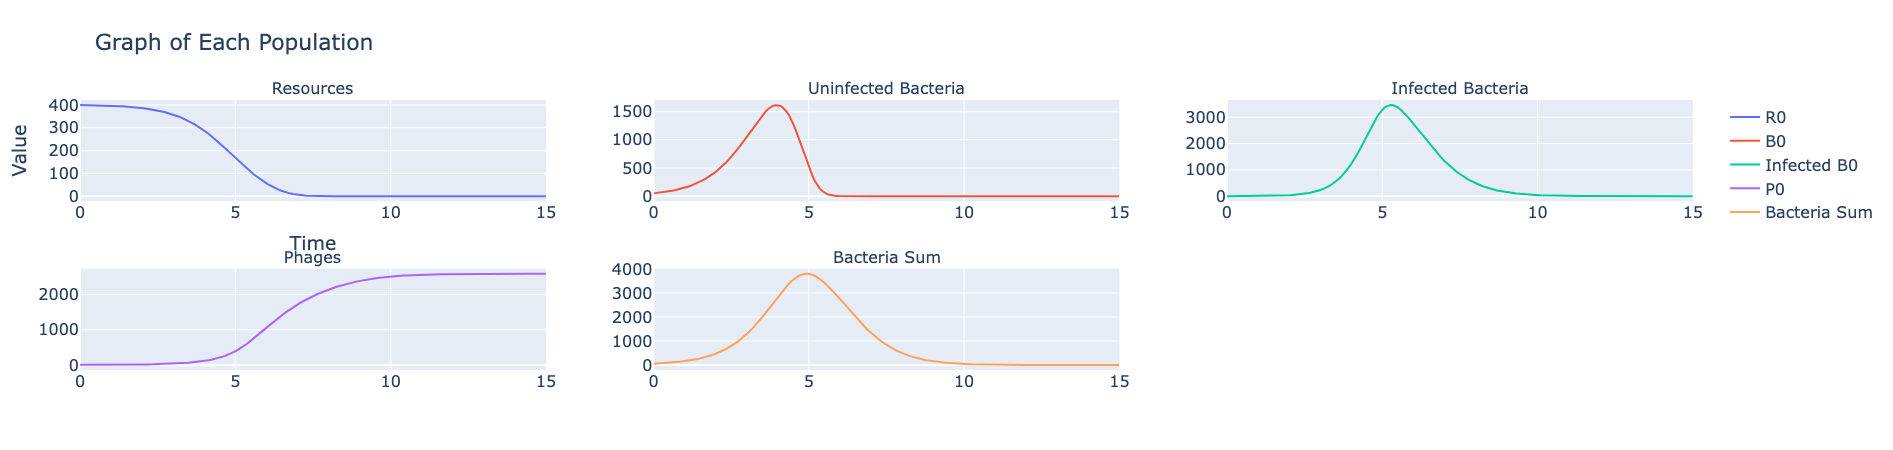
\includegraphics[width=\linewidth]{Plots/Created/a_good_curve_linear.png}
        \caption{
            Linear y-axis for a "good" plot. 
        }
        \label{fig:created:a_good_curve_linear}
    \end{subfigure}
    \hfill
    \begin{subfigure}{1\linewidth}
        \centering
        \captionsetup{width=1\linewidth}
        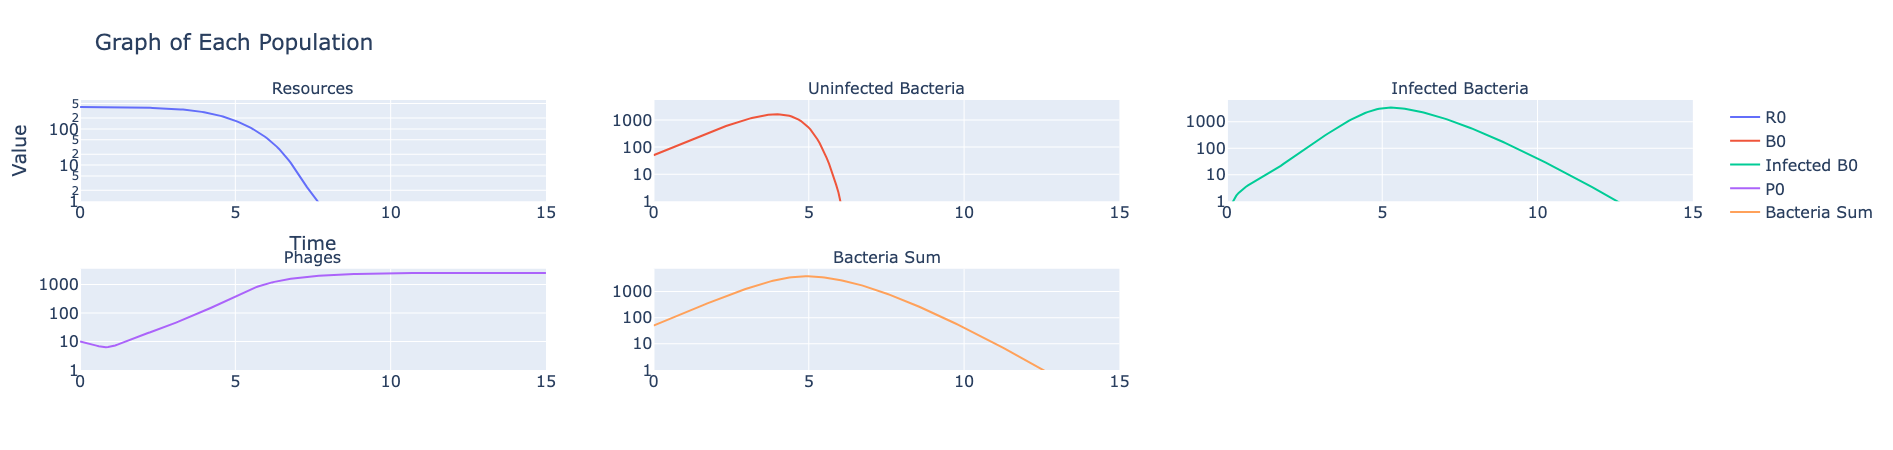
\includegraphics[width=\linewidth]{Plots/Created/a_good_curve_logarithmic.png}
        \caption{
            Logarithmic y-axis for a "good" plot. 
        }
        \label{fig:created:a_good_curve_logarithmic}
    \end{subfigure}
    \caption{The parameters used for this plot can be found in \Cref{tab:appendixE:a_good_curve}}
    \label{fig:created:a_good_curve}
\end{figure}



\section{SOBOL Sensitivity Analysis Results}
\label{sec:SOBOL_sensitivity_analysis_results}
It is important to understand how a change in parameter value affects the change in output of a model. 
Models will have parameters that are more important and have a larger effect on the model output than other parameters. 

\Cref{fig:created:SOBOL_average} shows the impact that the parameter had on the final value of the population at $t=15$. 
\Cref{fig:created:SOBOL_average} and \Cref{fig:created:SOBOL_variance} show the impact that the parameters had on the average value and variance of the population throughout the simulation respectively. 
The parameters that were tested include all the parameters listed in the extended golden model, except for Uninfected Bacteria and $M$. 
Uninfected Bacteria was left out as it doesn't make sense to already add infected bacteria to the system
$M$, the number of stages that the infection goes through, can not be tested as $M$ hardcodes the number of infection stages that the bacteria has to go through. 
The hardcoding is done before the simulation framework starts. 
As such, it is not possible to change $M$. 

What can immediately be noticed in \Cref{fig:created:SOBOL_default} is how the plots all look very similar. 
There might be some minor differences from bar to bar across plots, but the difference is imperceptible. 
SOBOL has some difficulty assigning a good sensitivity score to each parameter for the $ST$ and $S1$ tests. 
Resources, Uninfected, Phages, and Bacteria had more consistent results as seen by the smaller error bars. 

For the resources, the washin $\omega^i$ rate had the biggest influence on the final, average and variance value. 
Without a washin or washout rate, the resources would have most likely have been consumed by the time the simulation ended at $t=15$. 
The final values for resources, Uninfected, Infected, and Phages would often be something similar to (0, 0, 0, 10000), where all the resources were consumed and bacteria died out due to the phages, leaving only the phages remaining. 
So often the final value of the resources would be 0, no matter that the parameter values were. 
With the addition of the washin, new resources were constantly being re-added. 
Once the bacteria died out, the resources could accumulate, with the accumulation dependent on the rate of the washin rate, hence why the washin rate has such a large impact on the final, average, and variance of population value for the resources. 

The uninfected and infected populations had consistent outputs for the parameter inputs, where many parameter values were has an $ST \equiv 0.25$ for the Infected population. 
And since $ST_i >> S1_i$ for the uninfected and infected bacteria, the bacteria population are really dependent on higher order interactions. 
And looking at the golden model, this makes intuitive sense. 
The uninfected bacteria interact with $v$, $K$, $r$, $\omega^o$, while the infected bacteria interact with $\tau$ ($M$ is not included as it was left out of the analysis). 
These are 5 direct parameter interactions with more higher order interactions dependent on $\beta$, as the larger $\beta$ is, the faster the phage population can grow, the faster the bacteria become infected and die.   



\begin{figure}
    \centering
    \begin{subfigure}{0.32\linewidth}
        \centering
        \captionsetup{width=1\linewidth}
        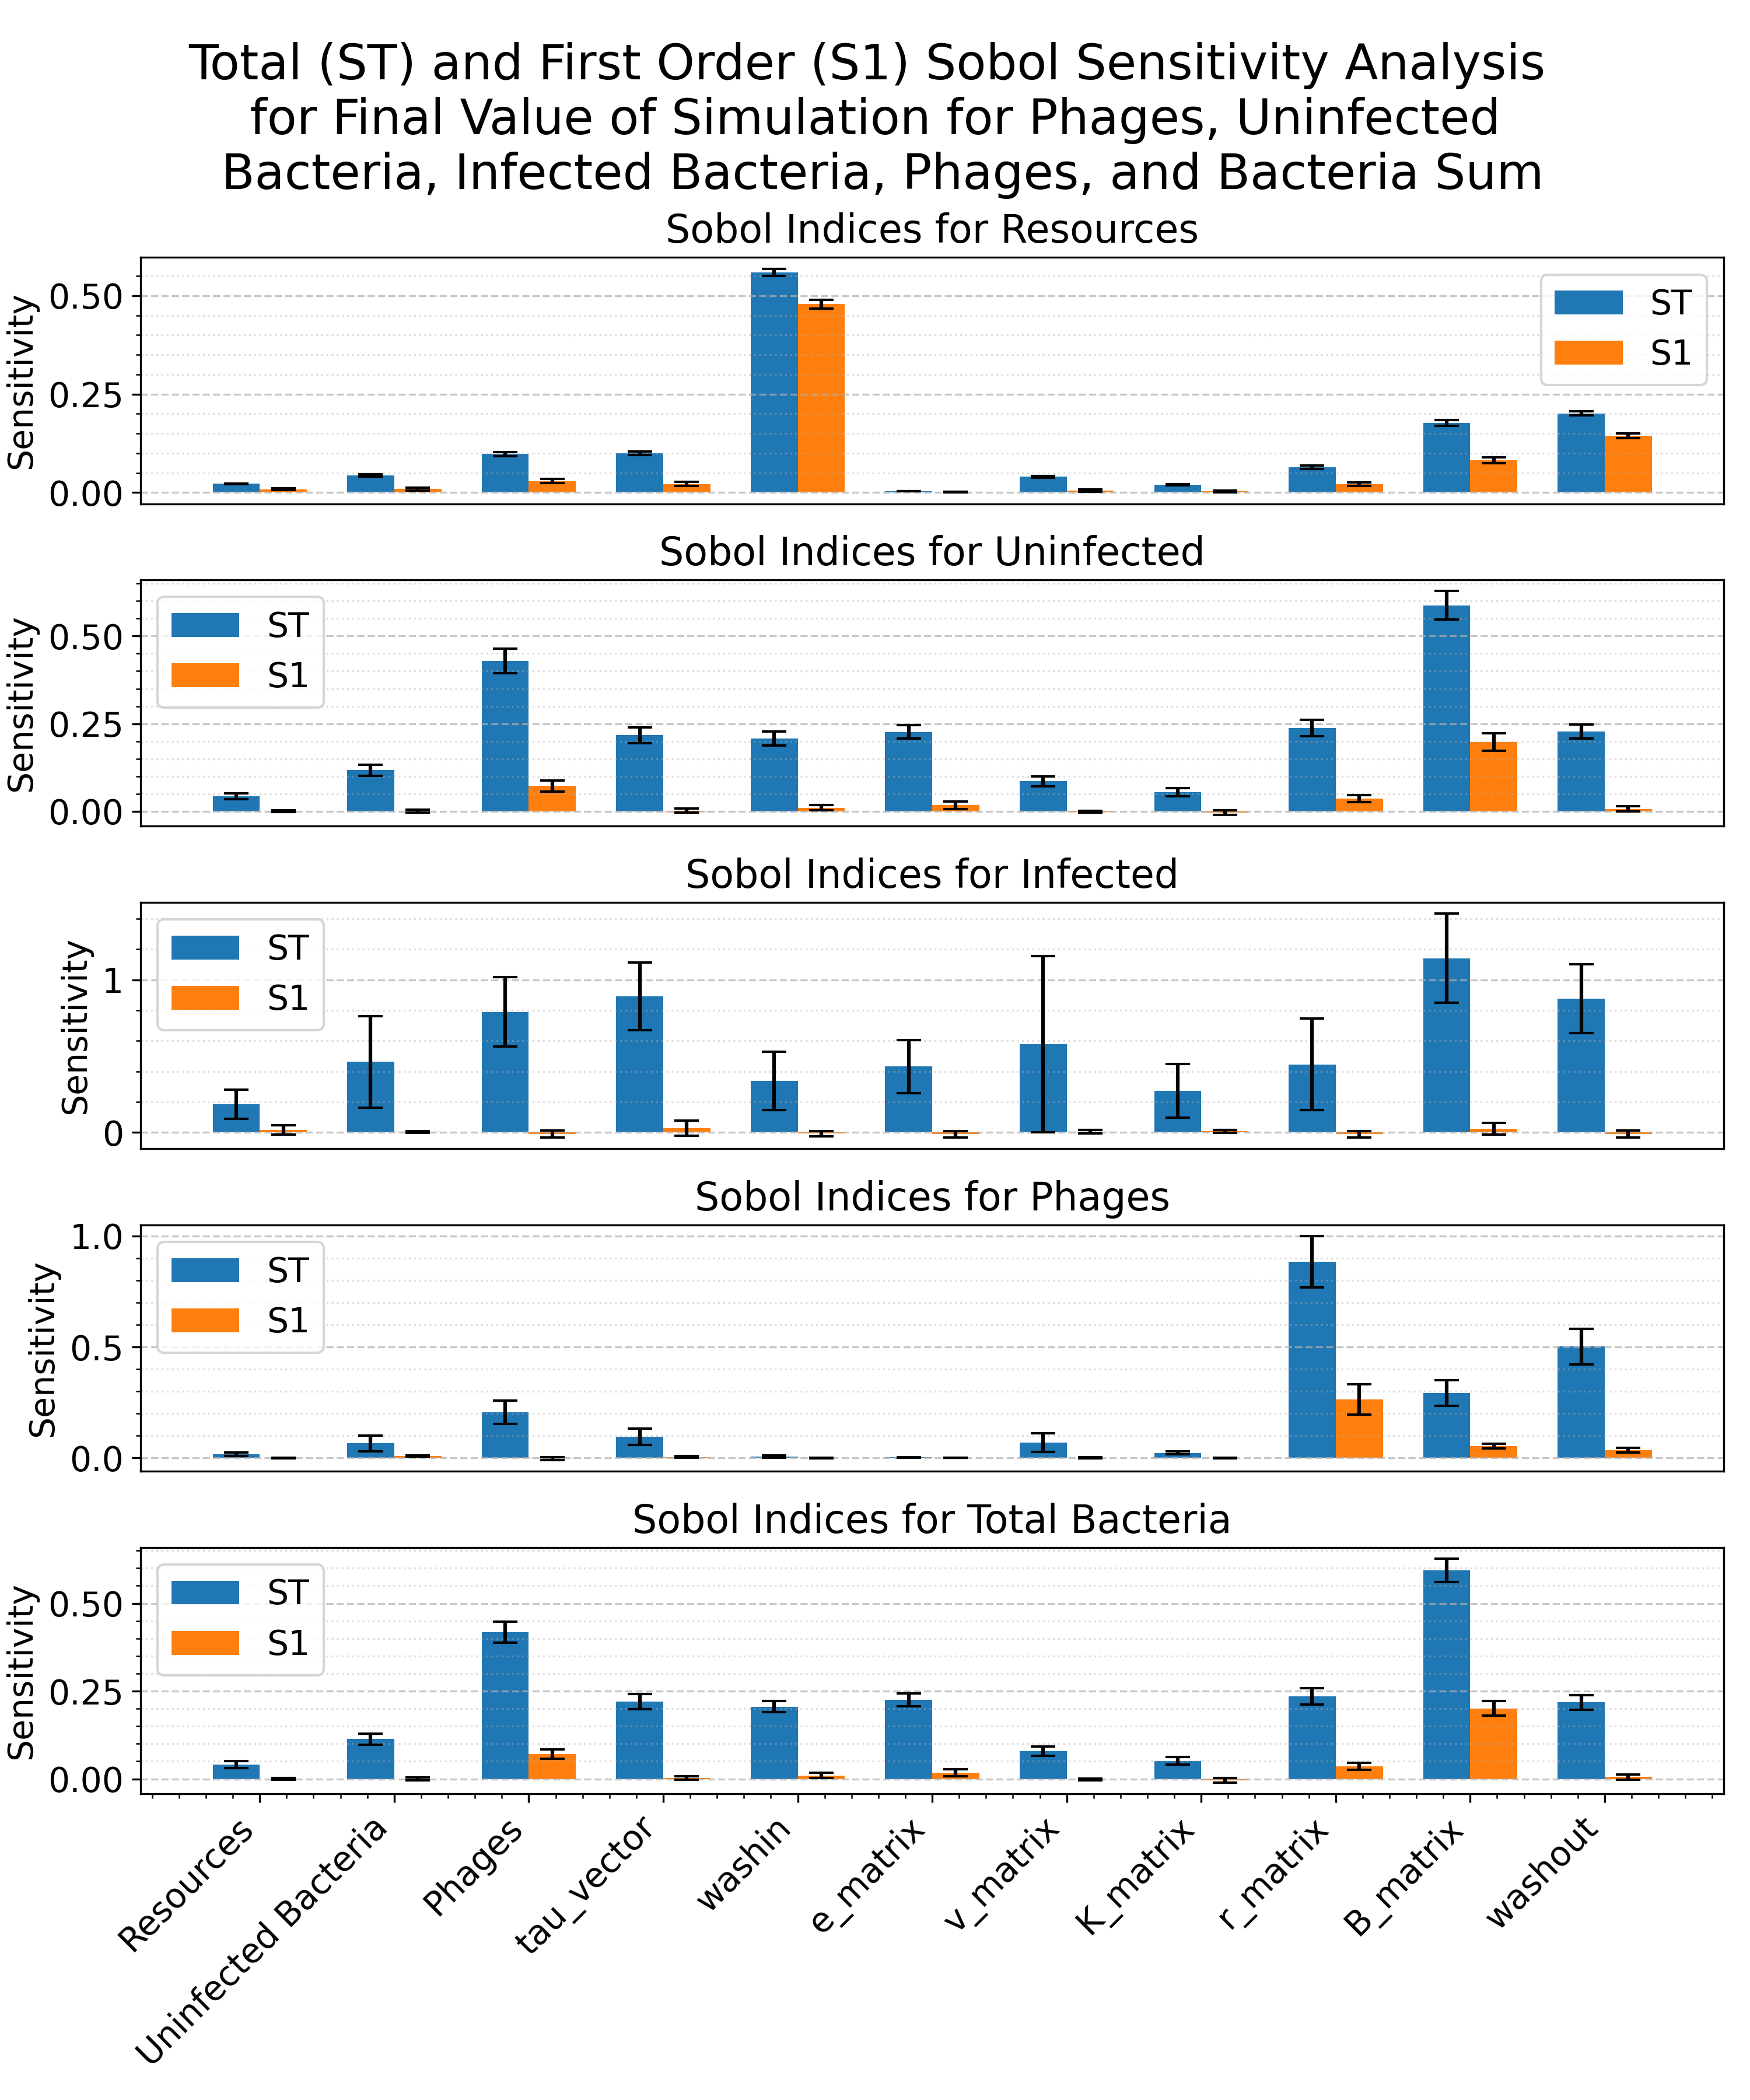
\includegraphics[width=\linewidth]{Plots/Created/SOBOL_analysis_1748084143_Final.png}
        \caption{
            The $ST$ and $S1$ sensitivity for the final Resource, Uninfected, Infected, Phage, and Total Bacteria population. 
        }
        \label{fig:created:SOBOL_final}
    \end{subfigure}
    \hfill
    \begin{subfigure}{0.32\linewidth}
        \centering
        \captionsetup{width=1\linewidth}
        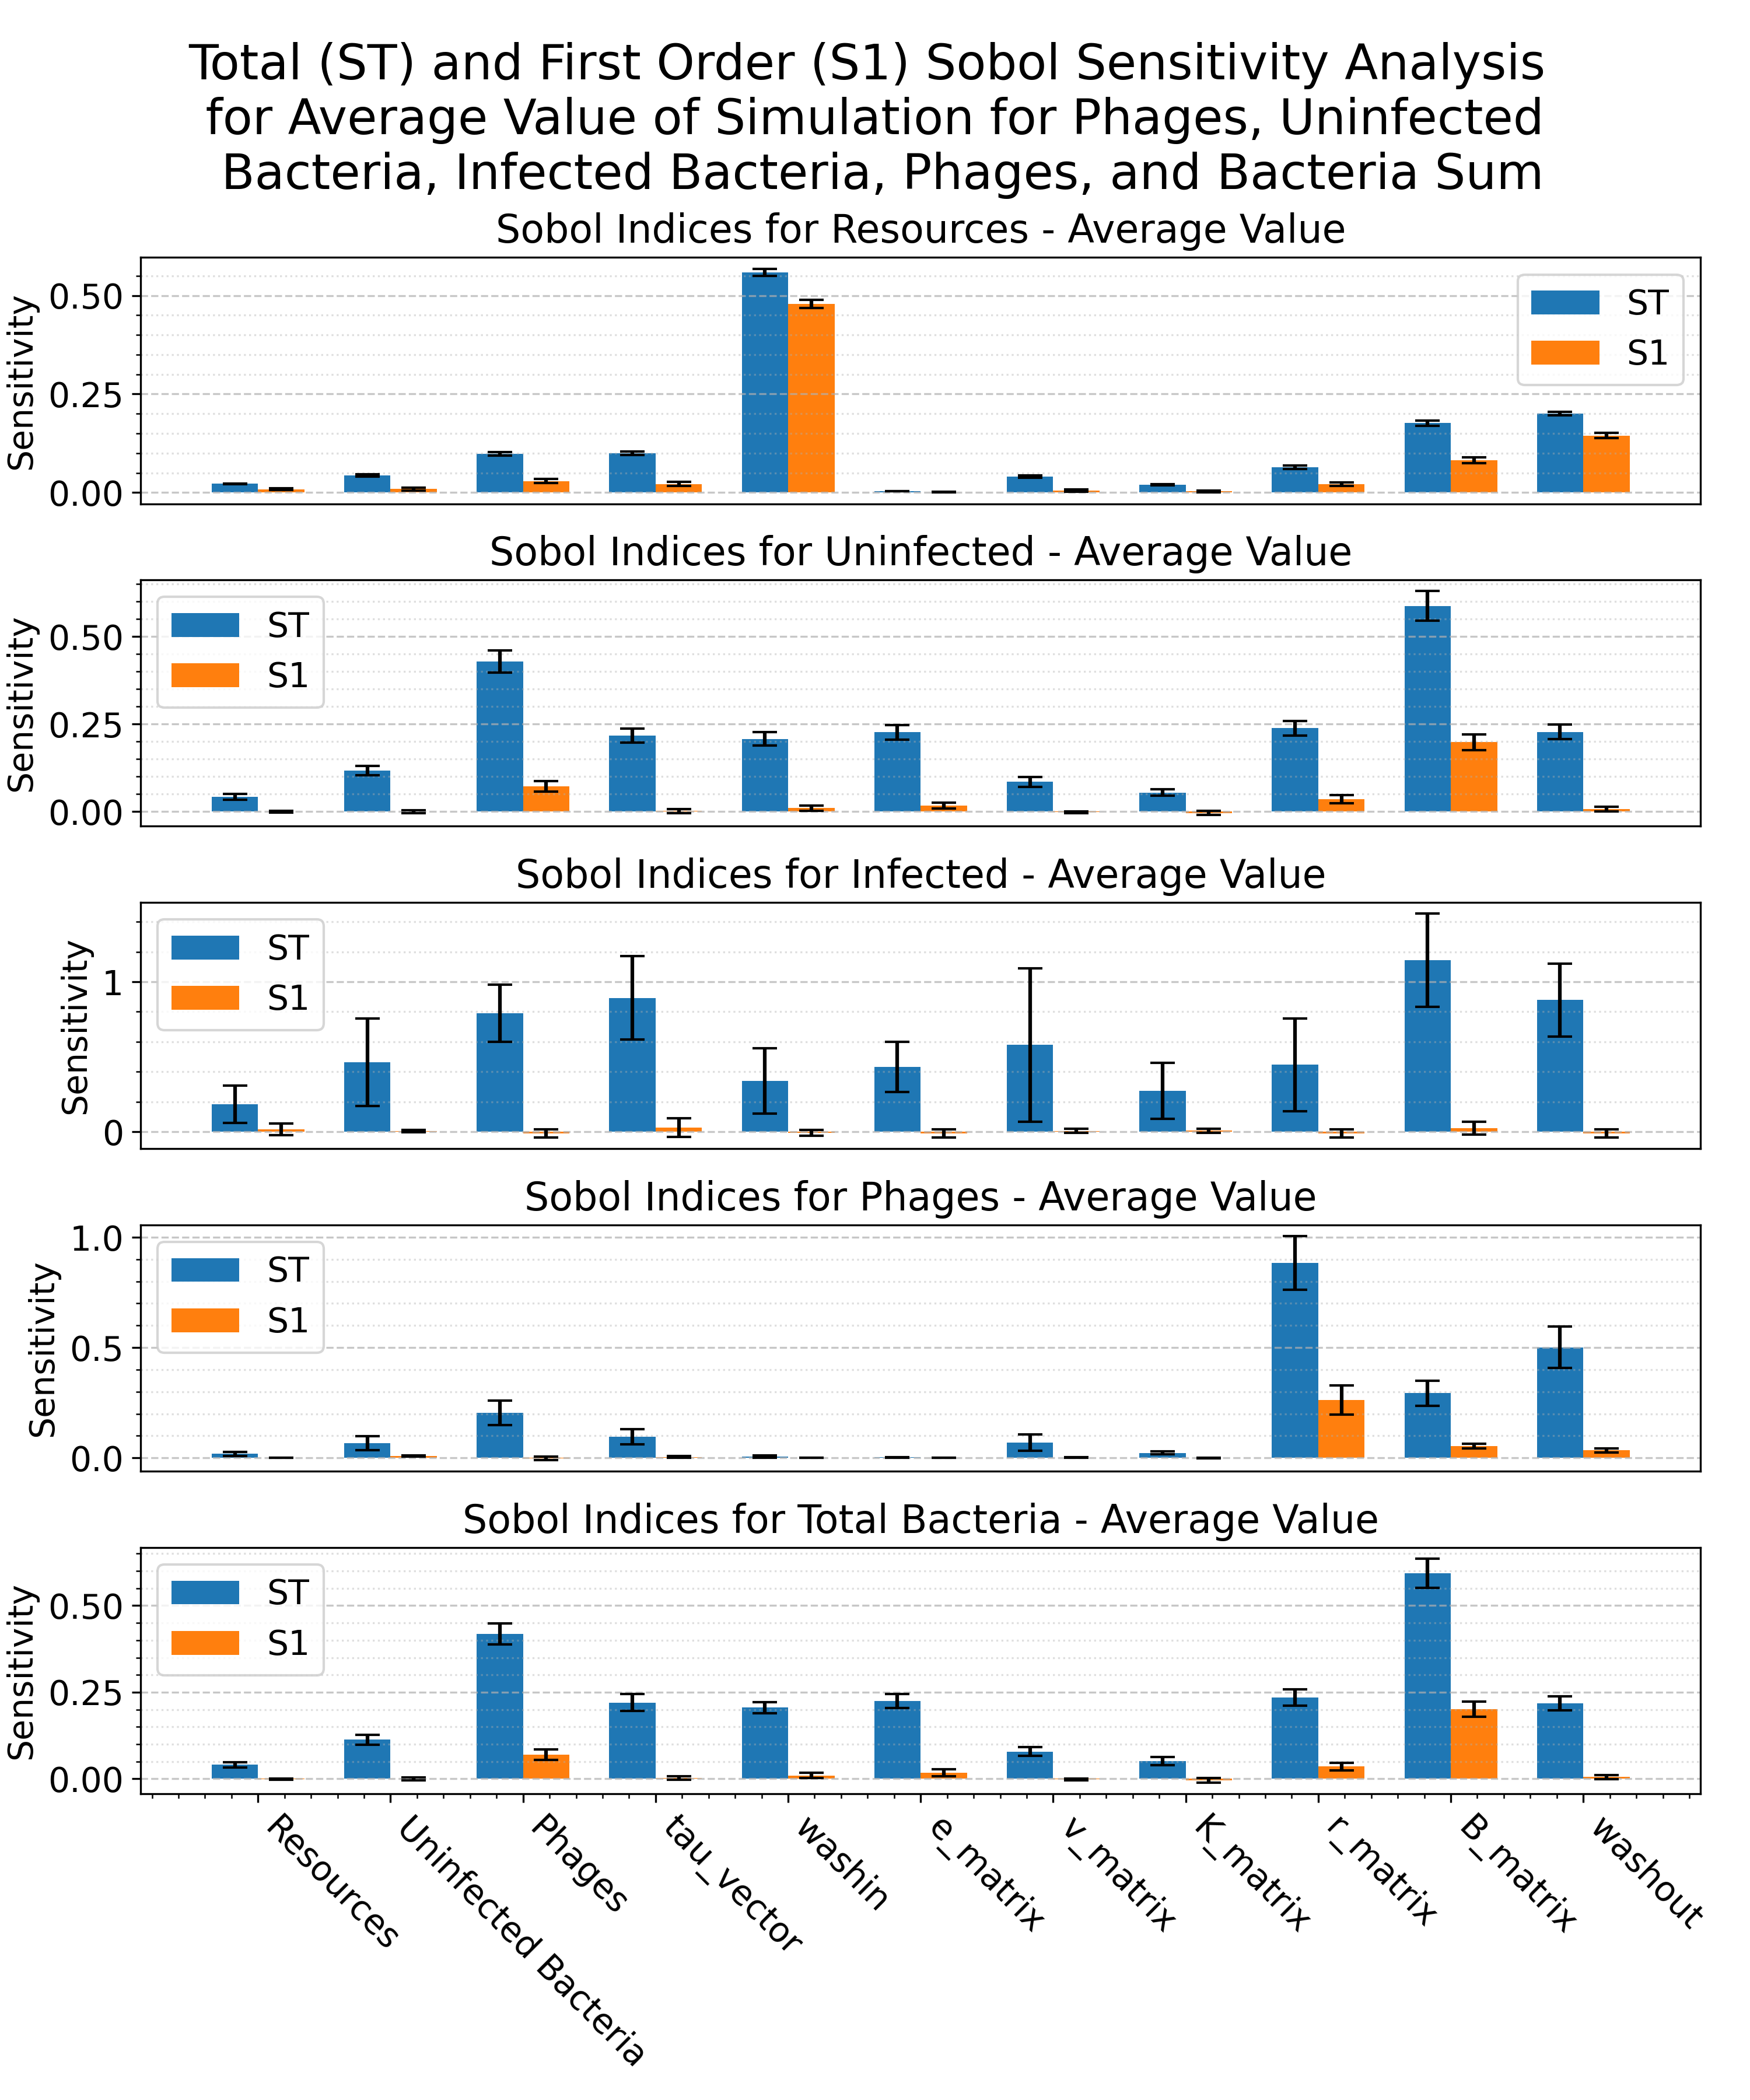
\includegraphics[width=\linewidth]{Plots/Created/SOBOL_analysis_1748084143_Average.png}
        \caption{
            The $ST$ and $S1$ order sensitivity for the average Resource, Uninfected, Infected, Phage, and Total Bacteria population. 
        }
        \label{fig:created:SOBOL_average}
    \end{subfigure}
    \hfill
    \begin{subfigure}{0.32\linewidth}
        \centering
        \captionsetup{width=1\linewidth}
        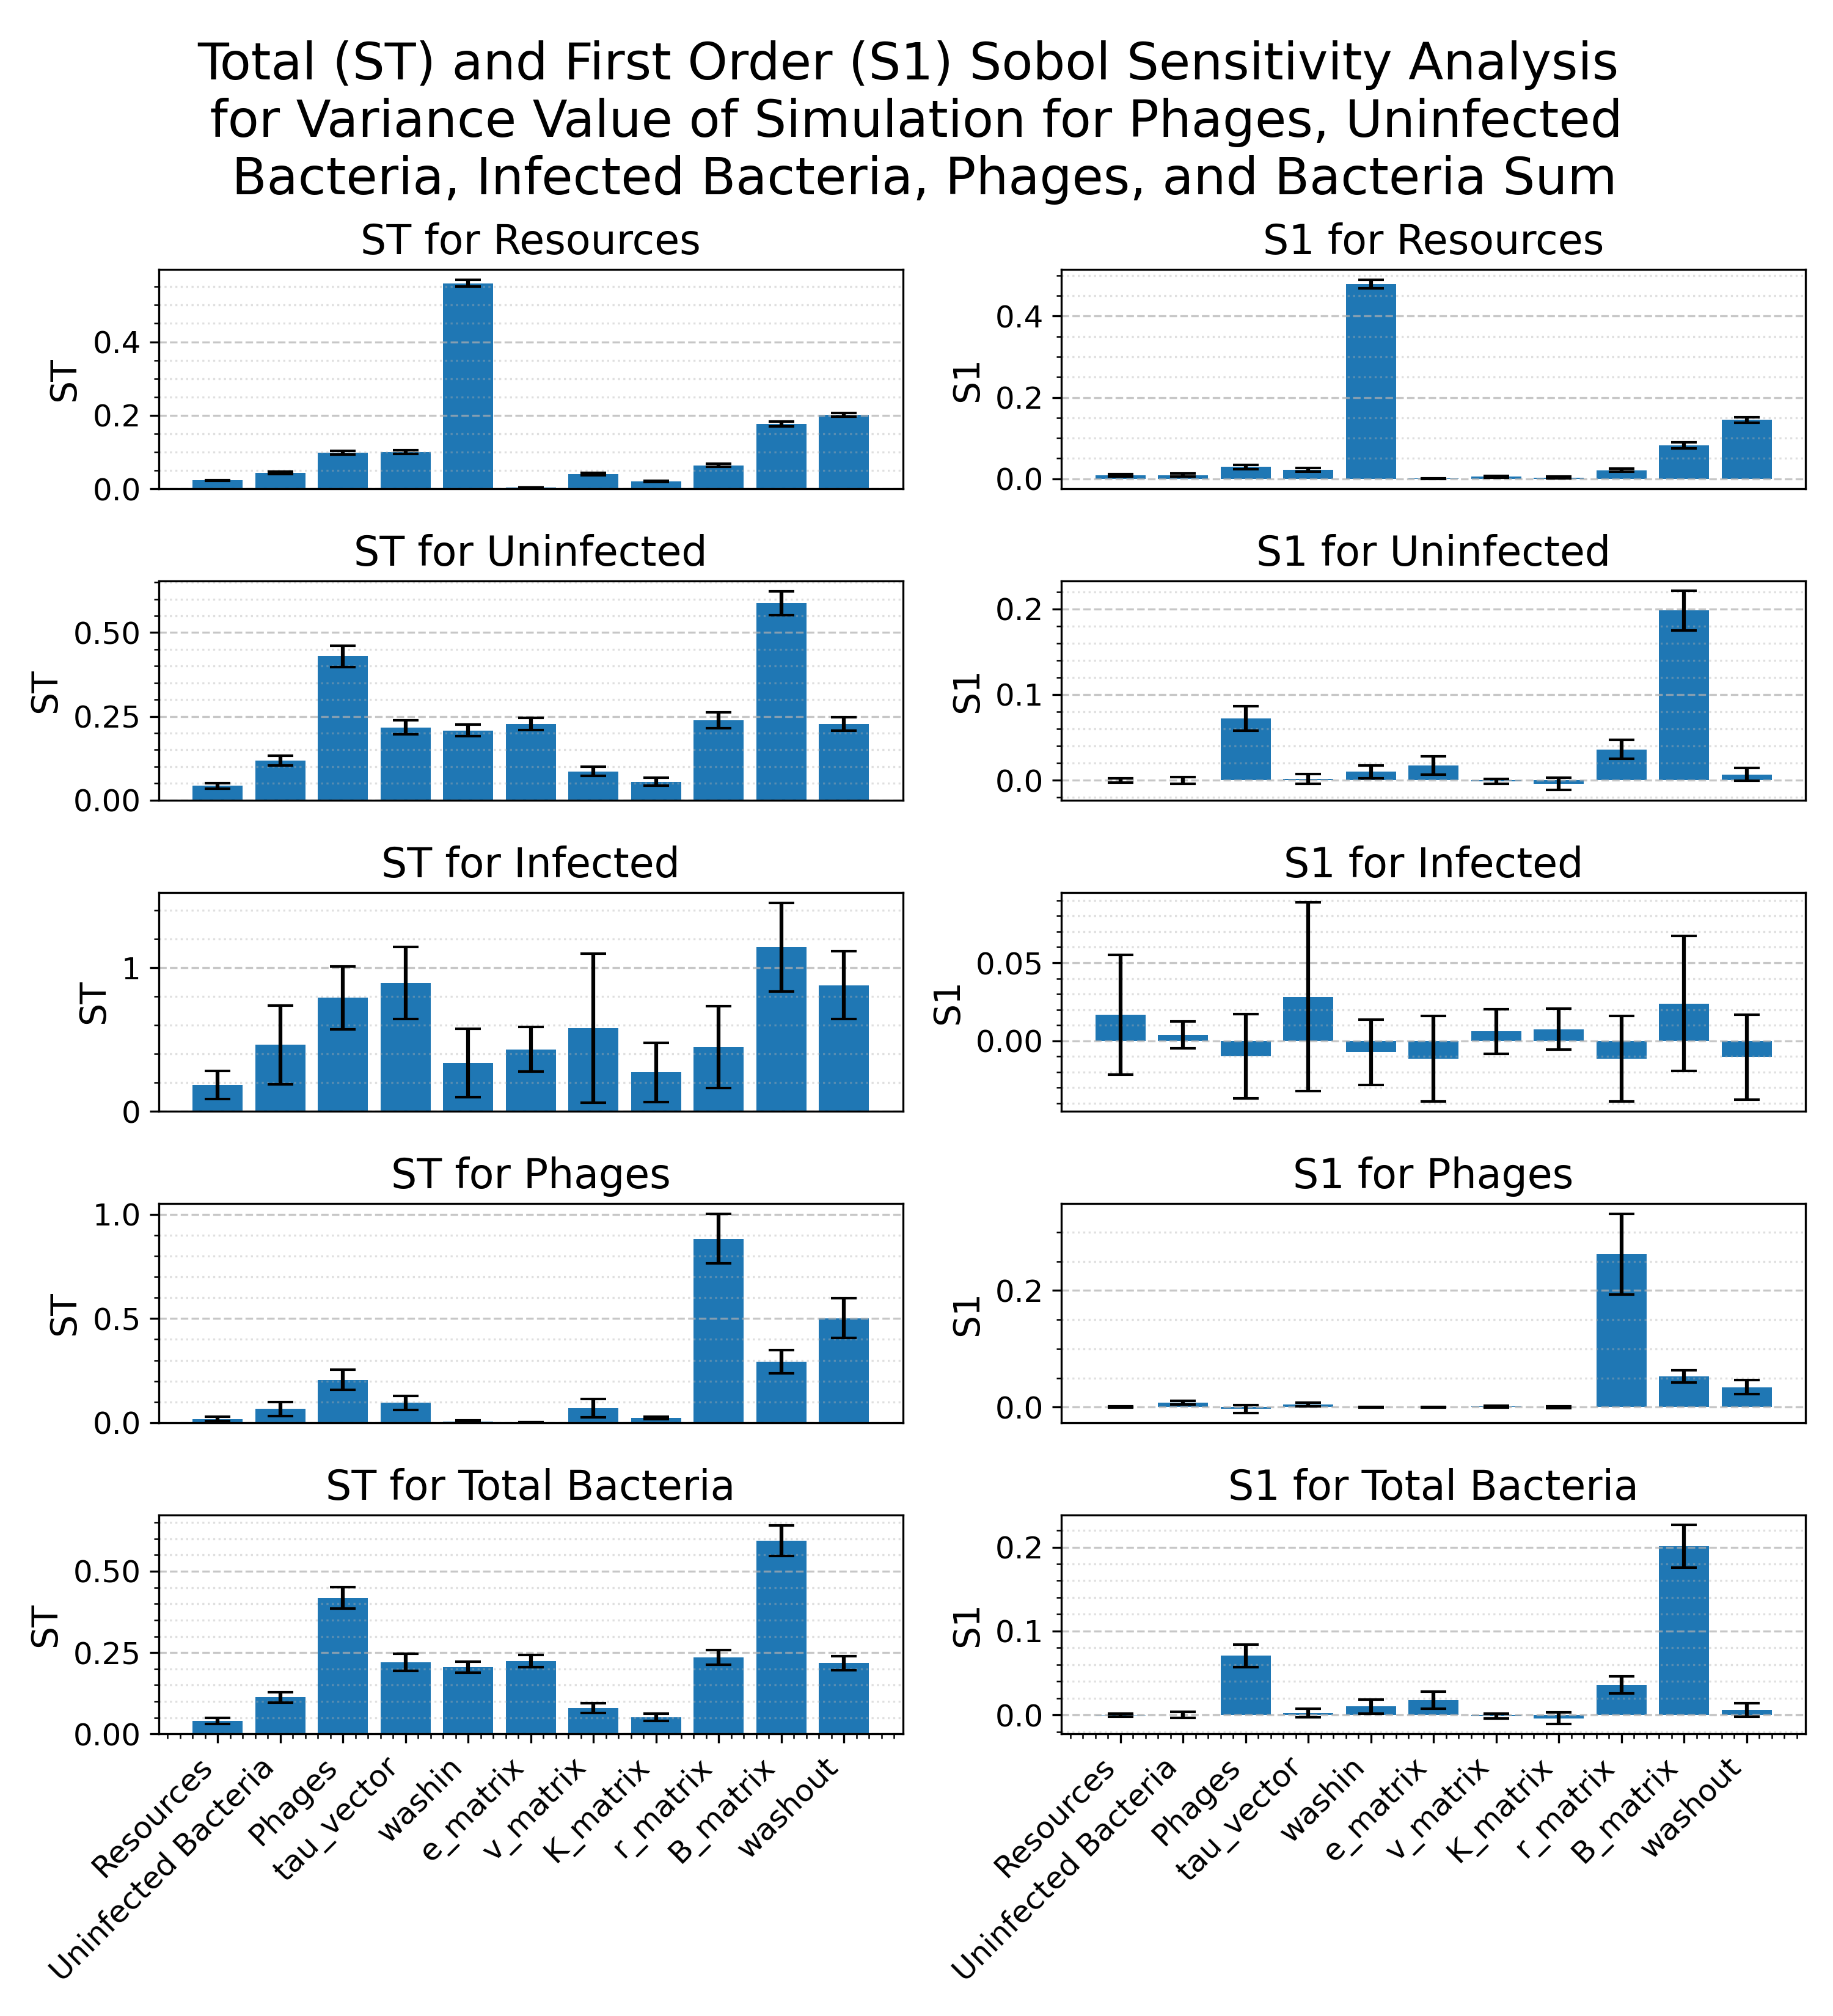
\includegraphics[width=\linewidth]{Plots/Created/SOBOL_analysis_1748084143_Variance.png}
        \caption{
            The $ST$ and $S1$ order sensitivity for the variance of Resource, Uninfected, Infected, Phage, and Total Bacteria. 
        }
        \label{fig:created:SOBOL_variance}
    \end{subfigure}
    \caption{
        The three default SOBOL analyses from the dashboard for the $1\times 1 \times 1$ golden model. 
        The data was saved from the dashboard and replotted using Matplotlib for a nicer plot and layout. 
        The values used for this SOBOL test can be found in \Cref{tab:appendixE:SOBOL_analysis_values}. 
        }
    \label{fig:created:SOBOL_default}
\end{figure}

\begin{figure}
    \centering
    \begin{subfigure}{0.49\linewidth}
        \centering
        \captionsetup{width=1\linewidth}
        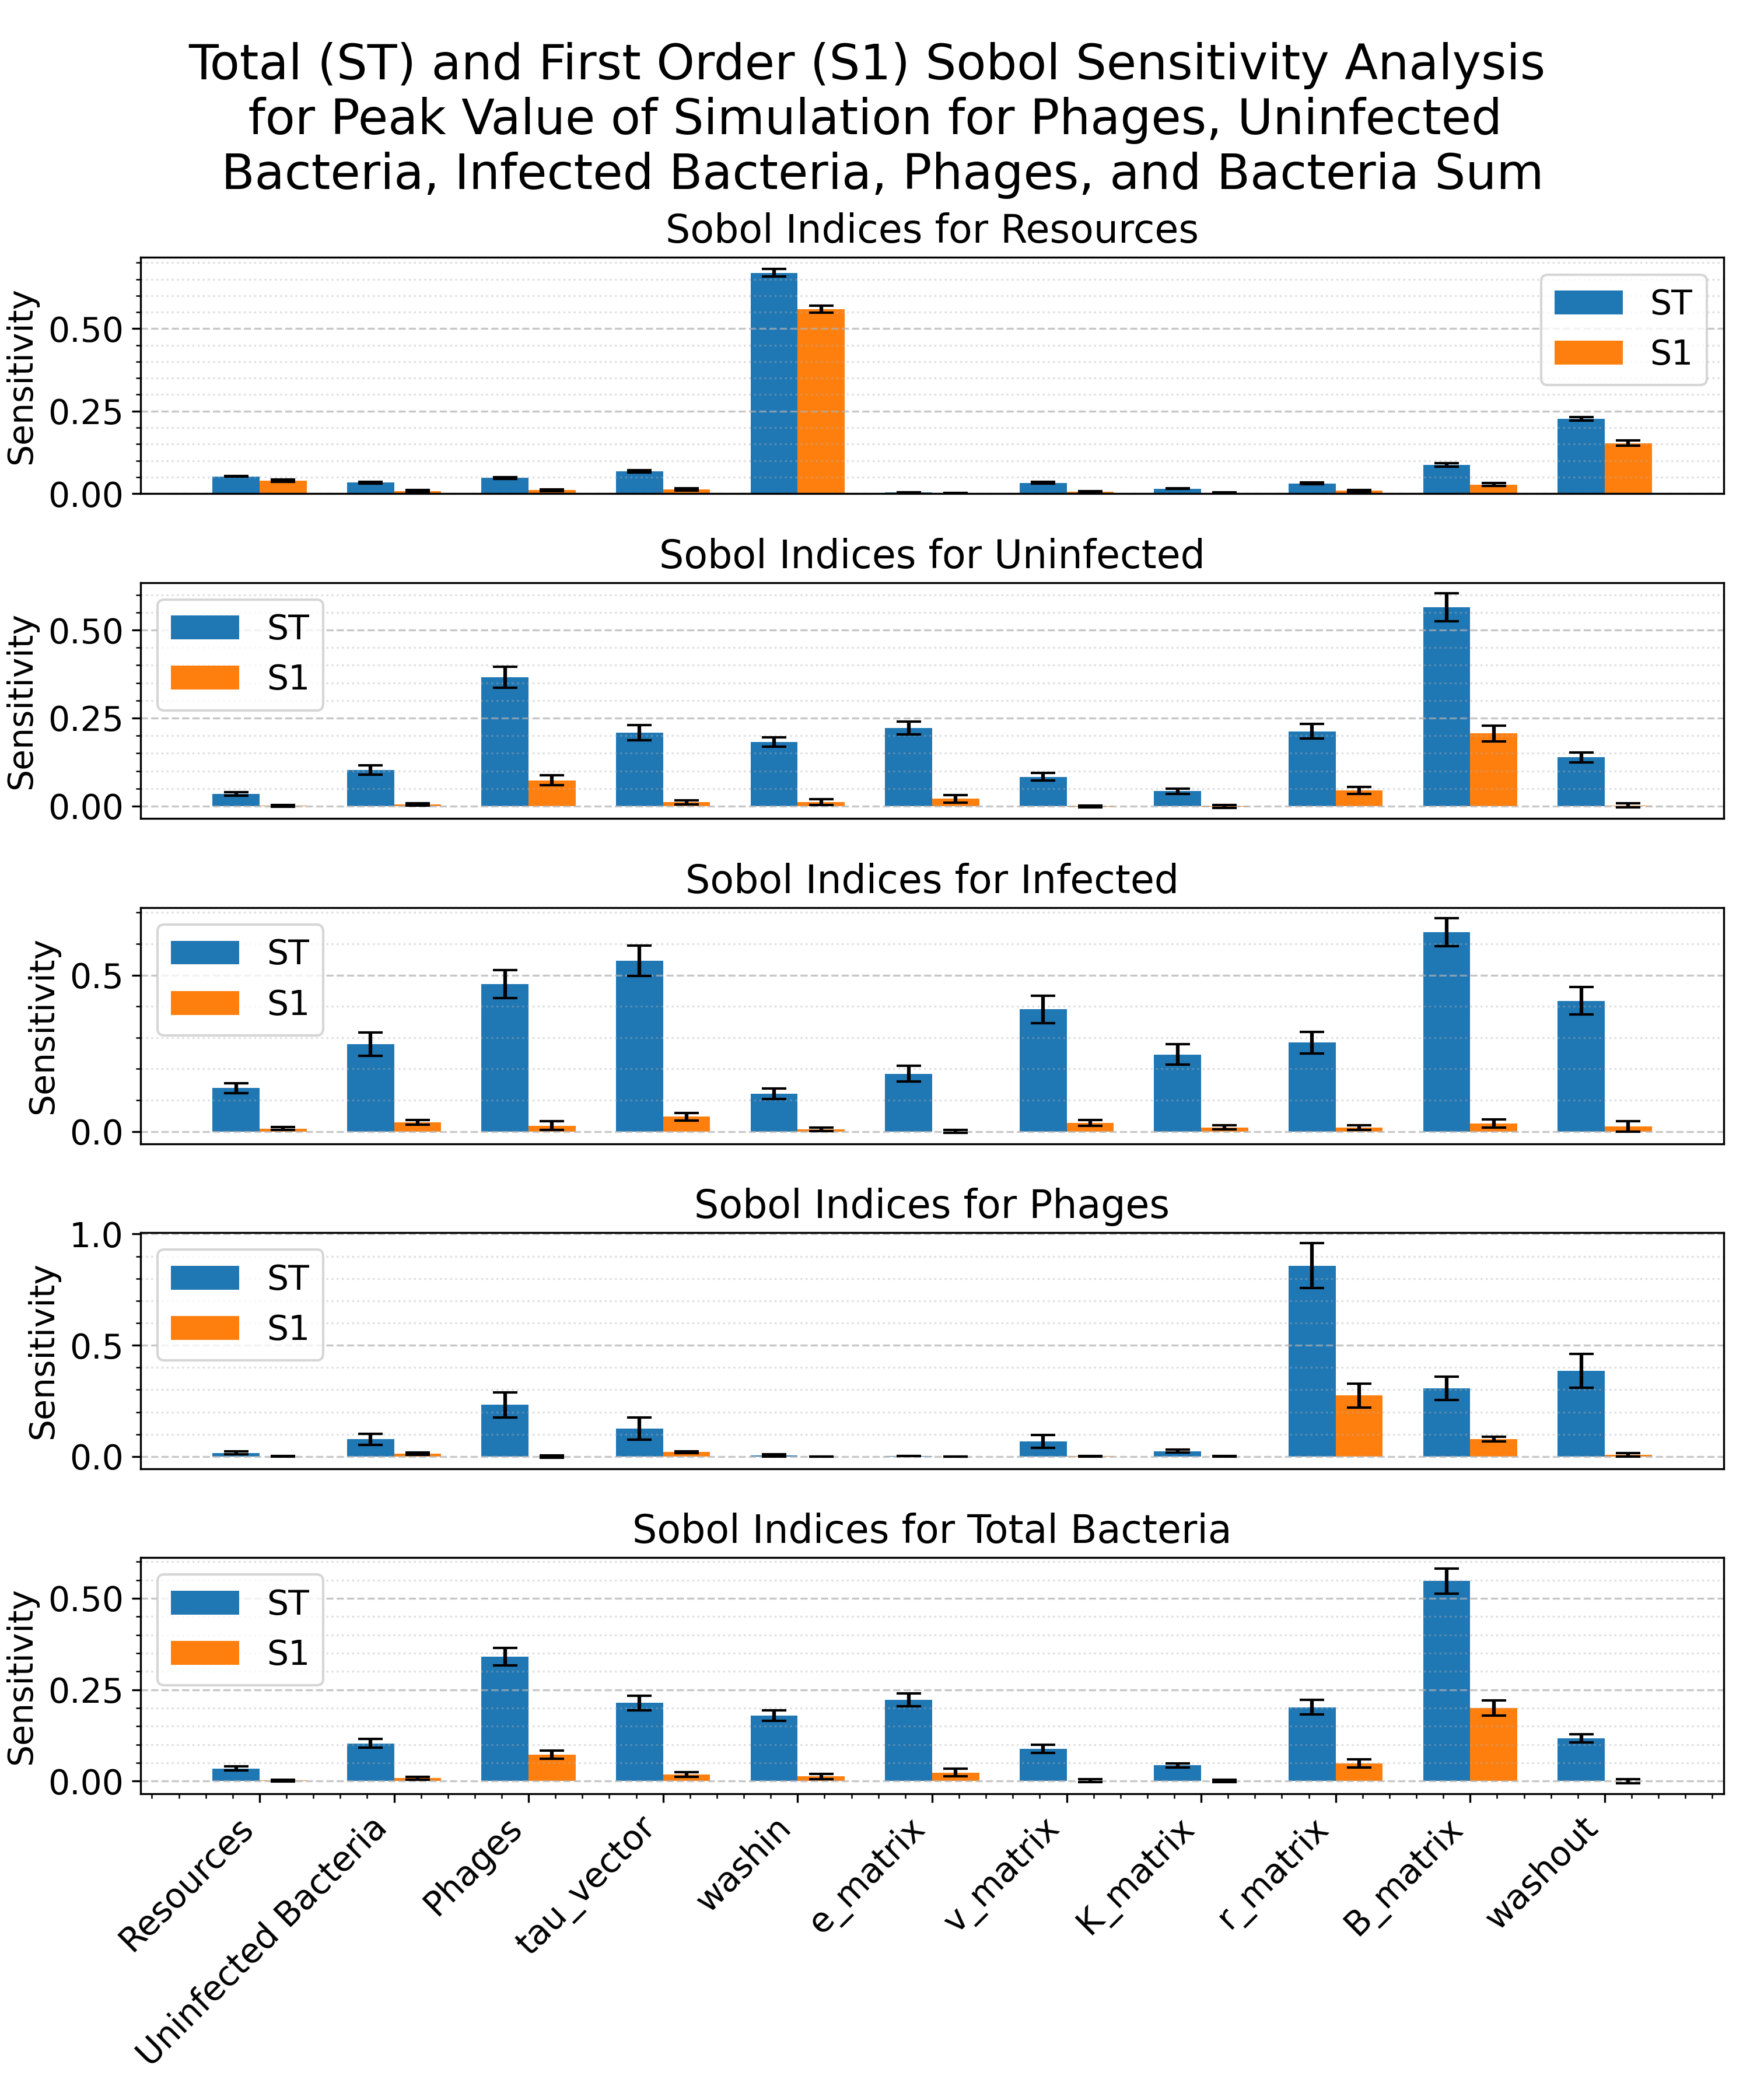
\includegraphics[width=\linewidth]{Plots/Created/SOBOL_analysis_1748084143_Peak.png}
        \caption{
            The total and first order sensitivity for the golden model for 95\% of the max value reached of the Resource, Uninfected, Infected, Phage, and Total Bacteria population count. 
        }
        \label{fig:created:SOBOL_peak}
    \end{subfigure}
    \hfill
    \begin{subfigure}{0.49\linewidth}
        \centering
        \captionsetup{width=1\linewidth}
        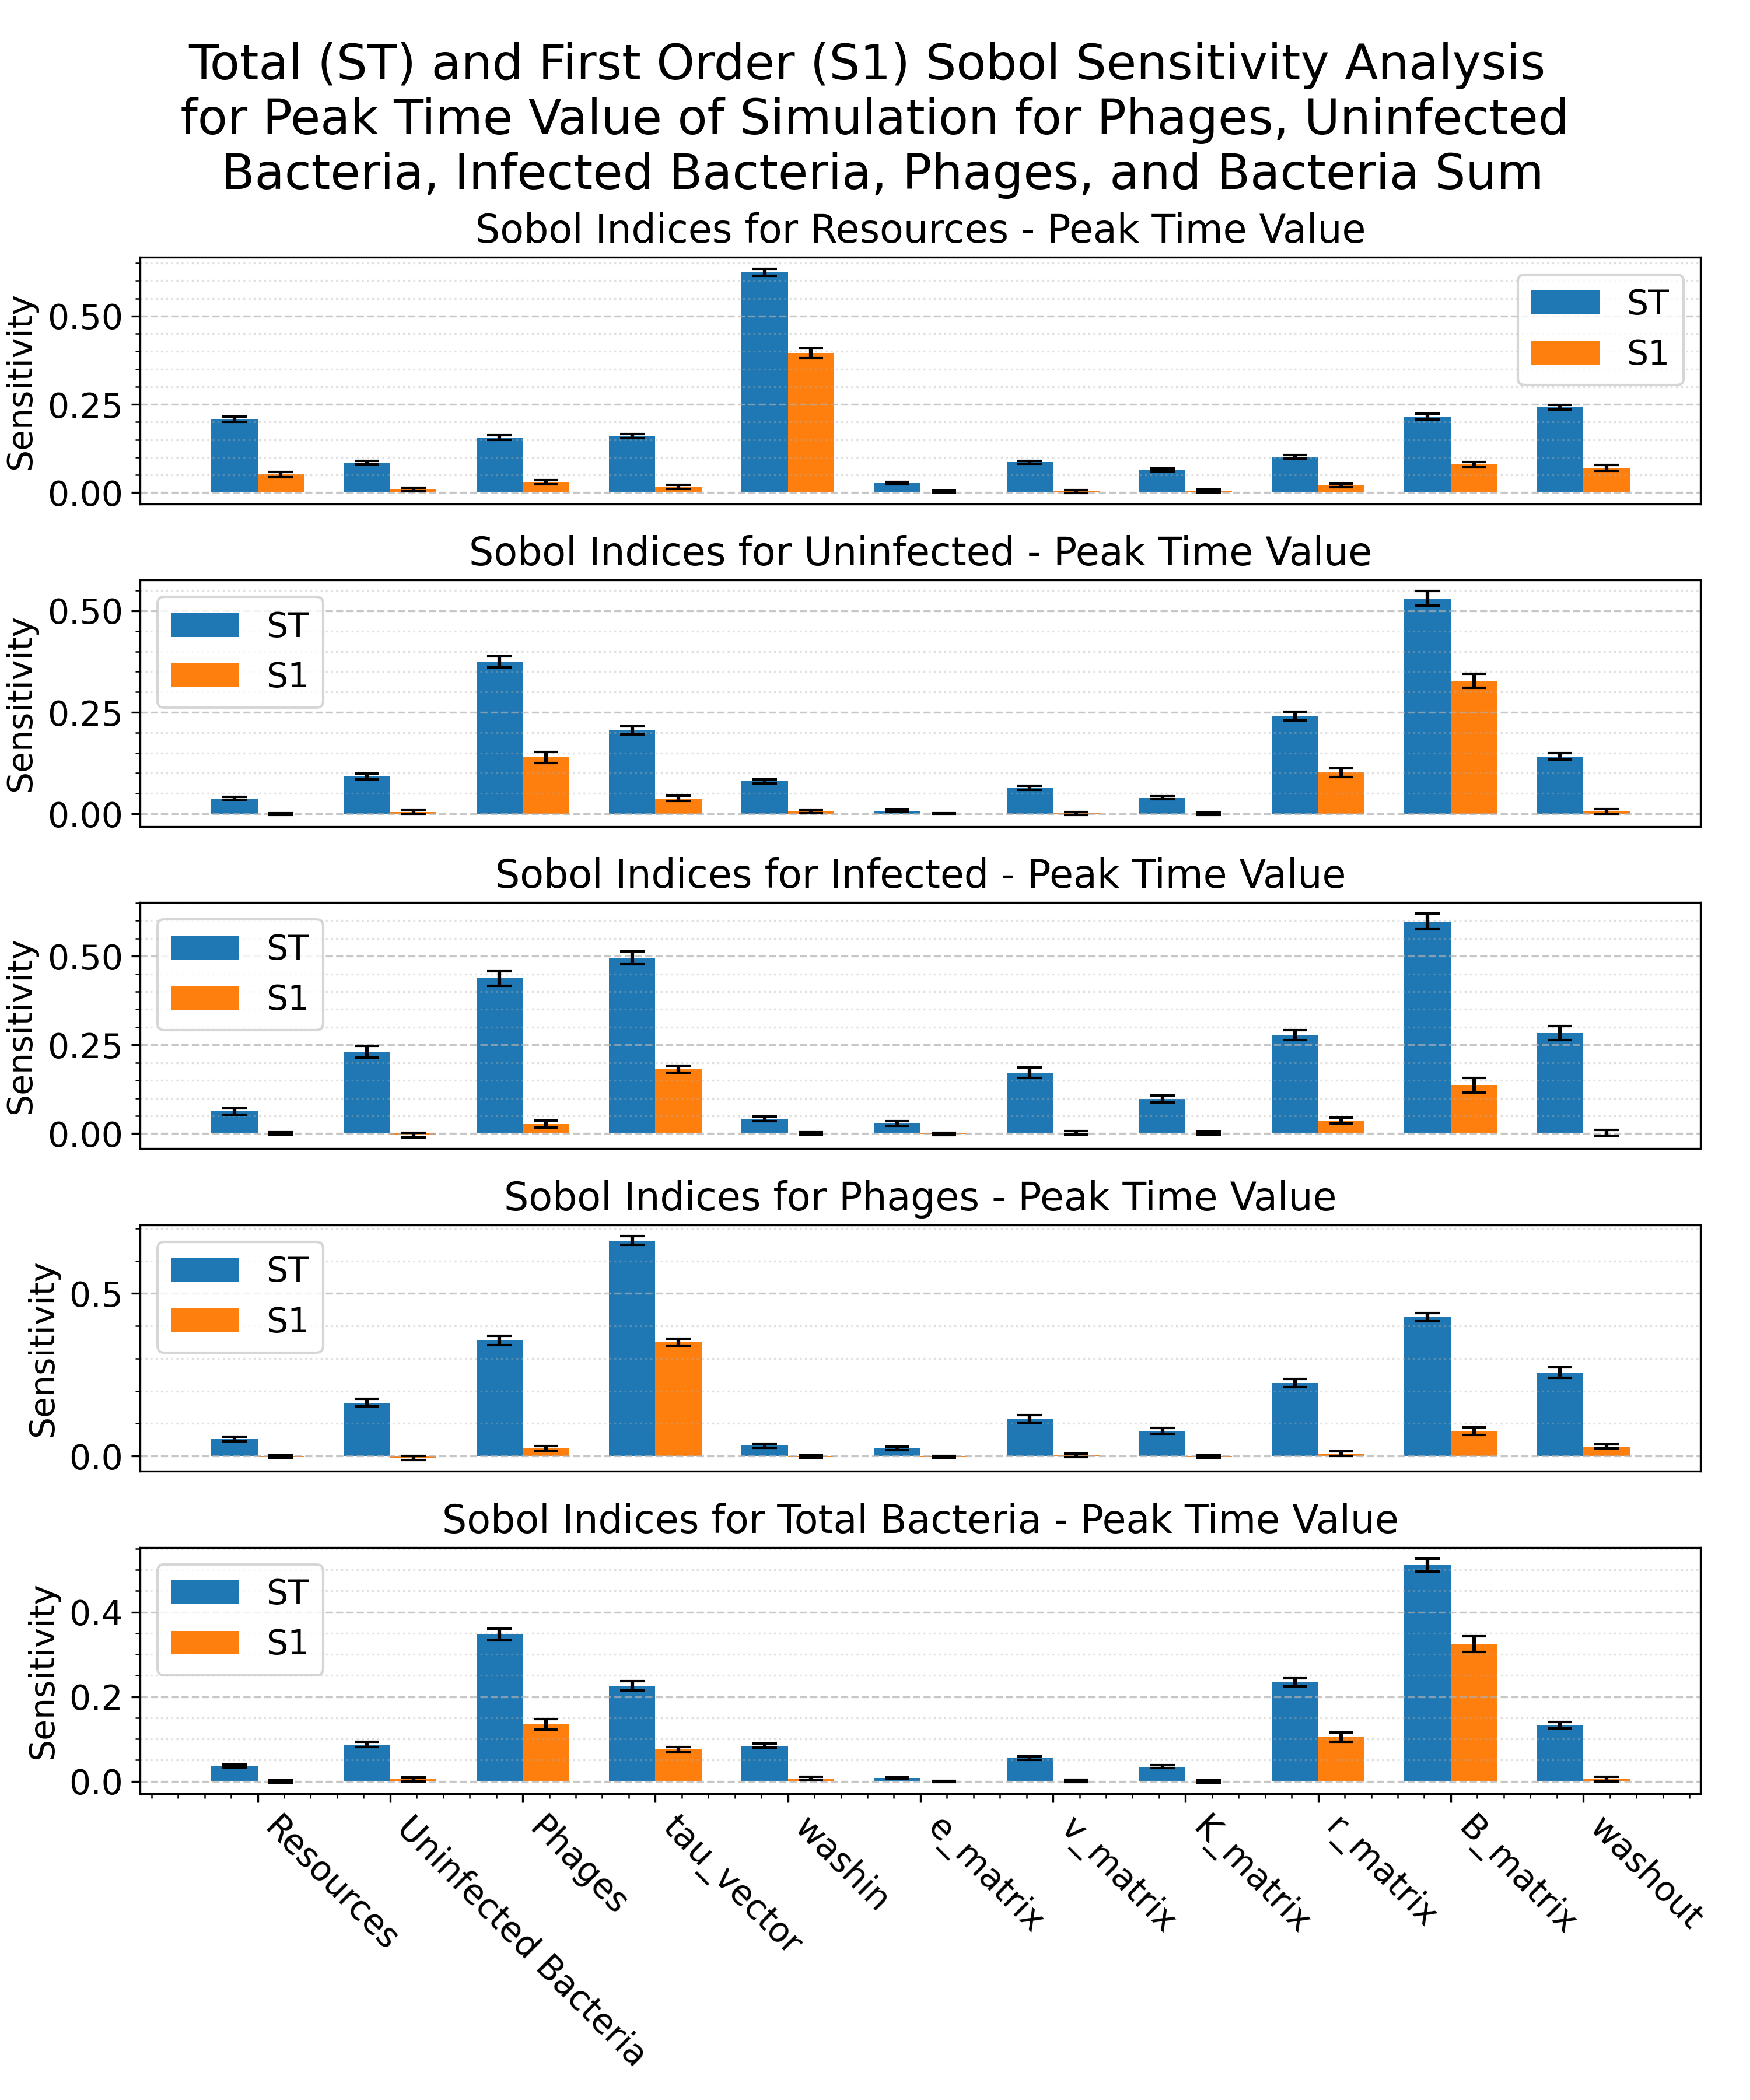
\includegraphics[width=\linewidth]{Plots/Created/SOBOL_analysis_1748084143_Peak_Time.png}
        \caption{
            The total and first order sensitivity for the golden model for the time at which 95\% of the max value occurred of the Resource, Uninfected, Infected, Phage, and Total Bacteria population value. 
        }
        \label{fig:created:SOBOL_peak_time}
        \end{subfigure}
    \caption{
        The three default SOBOL analyses from the dashboard for the $1\times 1 \times 1$ golden model. 
        The data was saved from the dashboard and replotted using Matplotlib for a nicer plot and layout. 
        The same values used in \Cref{fig:created:SOBOL_default} were used here, and a custom analysis was run on the saved data to create these plots. 
        The values used for this SOBOL test can be found in \Cref{tab:appendixE:SOBOL_analysis_values}. 
    }
    \label{fig:created:SOBOL_custom}
\end{figure}
